 \documentclass[10pt,aspectratio=169]{beamer}
\usetheme{Boadilla}

\usepackage{hyperref}
\usepackage{graphicx}
\usepackage{subfig}
\usepackage{xcolor}
\usepackage{amsmath,amssymb,physics}

\graphicspath{ {img/} }

\usepackage{tikz}

%Some useful commands for QM
%\newcommand{\bra}[1]{\left< #1 \right|}
%\newcommand{\ket}[1]{\left| #1 \right>}
%\newcommand{\expVal}[1]{\left< #1 \right>}
%\newcommand{\braket}[2]{\left<#1|#2\right>}

% Set beamer color info
\definecolor{BOrange}{RGB}{191,87,0}
\setbeamercolor{title}{fg=black}
\setbeamercolor{frametitle}{fg=black}
\setbeamercolor{structure}{fg=BOrange}

%Stolen from http://tex.stackexchange.com/questions/178800/creating-sections-each-with-title-pages-in-beamers-slides
%\AtBeginSection[]{
%  \begin{frame}
%  \vfill
%  \centering
%  \begin{beamercolorbox}[sep=8pt,center,shadow=true,rounded=true]{title}
%    \usebeamerfont{title}\insertsectionhead\par%
%  \end{beamercolorbox}
%  \vfill
%  \end{frame}
%}

\title{The Speed of Quantum Information Spreading in
Chaotic Systems}
\subtitle{Work with Stefan Eccles, Phuc Nguyen, Brian Swingle, and Shenglong Xu\\ arxiv:1908.06993}
\author{Josiah Couch}
\institute{University of Texas at Austin}
\date{11 December 2019}


% Title frame
\begin{document}

\begin{frame}
\titlepage

\end{frame}

% Introduction
\begin{frame}
\frametitle{Punchline}

\begin{itemize}

\item We study the speed at which initially local quantum information spreads, i.e., the {\it information velocity}.

\item When this information is entanglement with some reference, this can be defined as the rate of growth of the smallest region whose mutual information with that reference is maximal.

\item For a chaotic translationally invariant system after a quench, we claim

\begin{equation}
v_I = \frac{v_E(f)}{1-f}
\end{equation}

\item where

	\begin{itemize}
	
	\item $v_E$ is the entanglement velocity
	
	\item $f$ is the ratio of the entropy density immediately after the quench to that in the asymptotic future.
	
	\end{itemize}
	
\item This claim is supported by a general quantum information argument, spin chain numerics, and a holographic computation.

\end{itemize}

\end{frame}

% Outline
\begin{frame}
\frametitle{Outline}

\begin{itemize}

\item The Setup

\item General Quantum Information Argument

\item Computations for specific systems

	\begin{itemize}
	
	\item Spin Chain 
	
	\item Holography	
	
	\end{itemize}
	
\item Overview of results

\end{itemize}

\end{frame}

% Setup
\begin{frame}
\frametitle{Setup}

\begin{itemize}

\item Consider a chaotic quantum system along with a reference system.

\item Let $\ket{\psi}$ be a translation-invariant state with fixed energy density $\epsilon$. $\ket{\psi}$ may not be in equilibrium, in which case the entropy density will be increasing. 

\item We assume that the entanglement entropy of any large region $A$ at a given time $t$ is given to leading order by

\begin{equation}
S(A) = \min \bigg(s |A|, s \left(f |A| + v_E |\partial A| t \right) \bigg)
\end{equation}

\item Assume that for a local perturbation $W$, the Heisenberg operator $W(t)$ approximately has support on a region of size $v_B t$

\item Assume that we can think of our Hilbert space as a tensor product of Hilbert spaces on subregions of size $\xi$, where $\xi$ is the correlation length.

\item Assume that $v_B$ is the fastest velocity in our system (at this energy density).

\item At a time $t_0$, we will maximally entangle the reference system to some degrees of freedom localized to a small region.

\end{itemize}

\end{frame}

% QI Argument

% Hayden-Preskill
\begin{frame}
\frametitle{Quantum Information Argument: Hayden-Preskill}

\begin{minipage}[t]{0.44\linewidth}

\begin{itemize}

\item QI argument is based on a generalization of Hayden-Preskill (2007).

\item HP has 3 systems: a reference R, a memory M, and a system S, where $|M| > |S|$.

\item R is initially entangled with a small subsystem of S. The rest of S is maximally entangled with M.

\item S then evolves by a random unitary

\item After evolution, M plus a small subsystem of S is enough to recover entanglement with R.

\item Our generalization breaks down into two cases: $f=1$ (saturated) and $f<1$ (unsaturated). 

\end{itemize}

\end{minipage}\hfill
%
\begin{minipage}[t]{0.55\linewidth}

\begin{figure}
    \begin{center}
    
        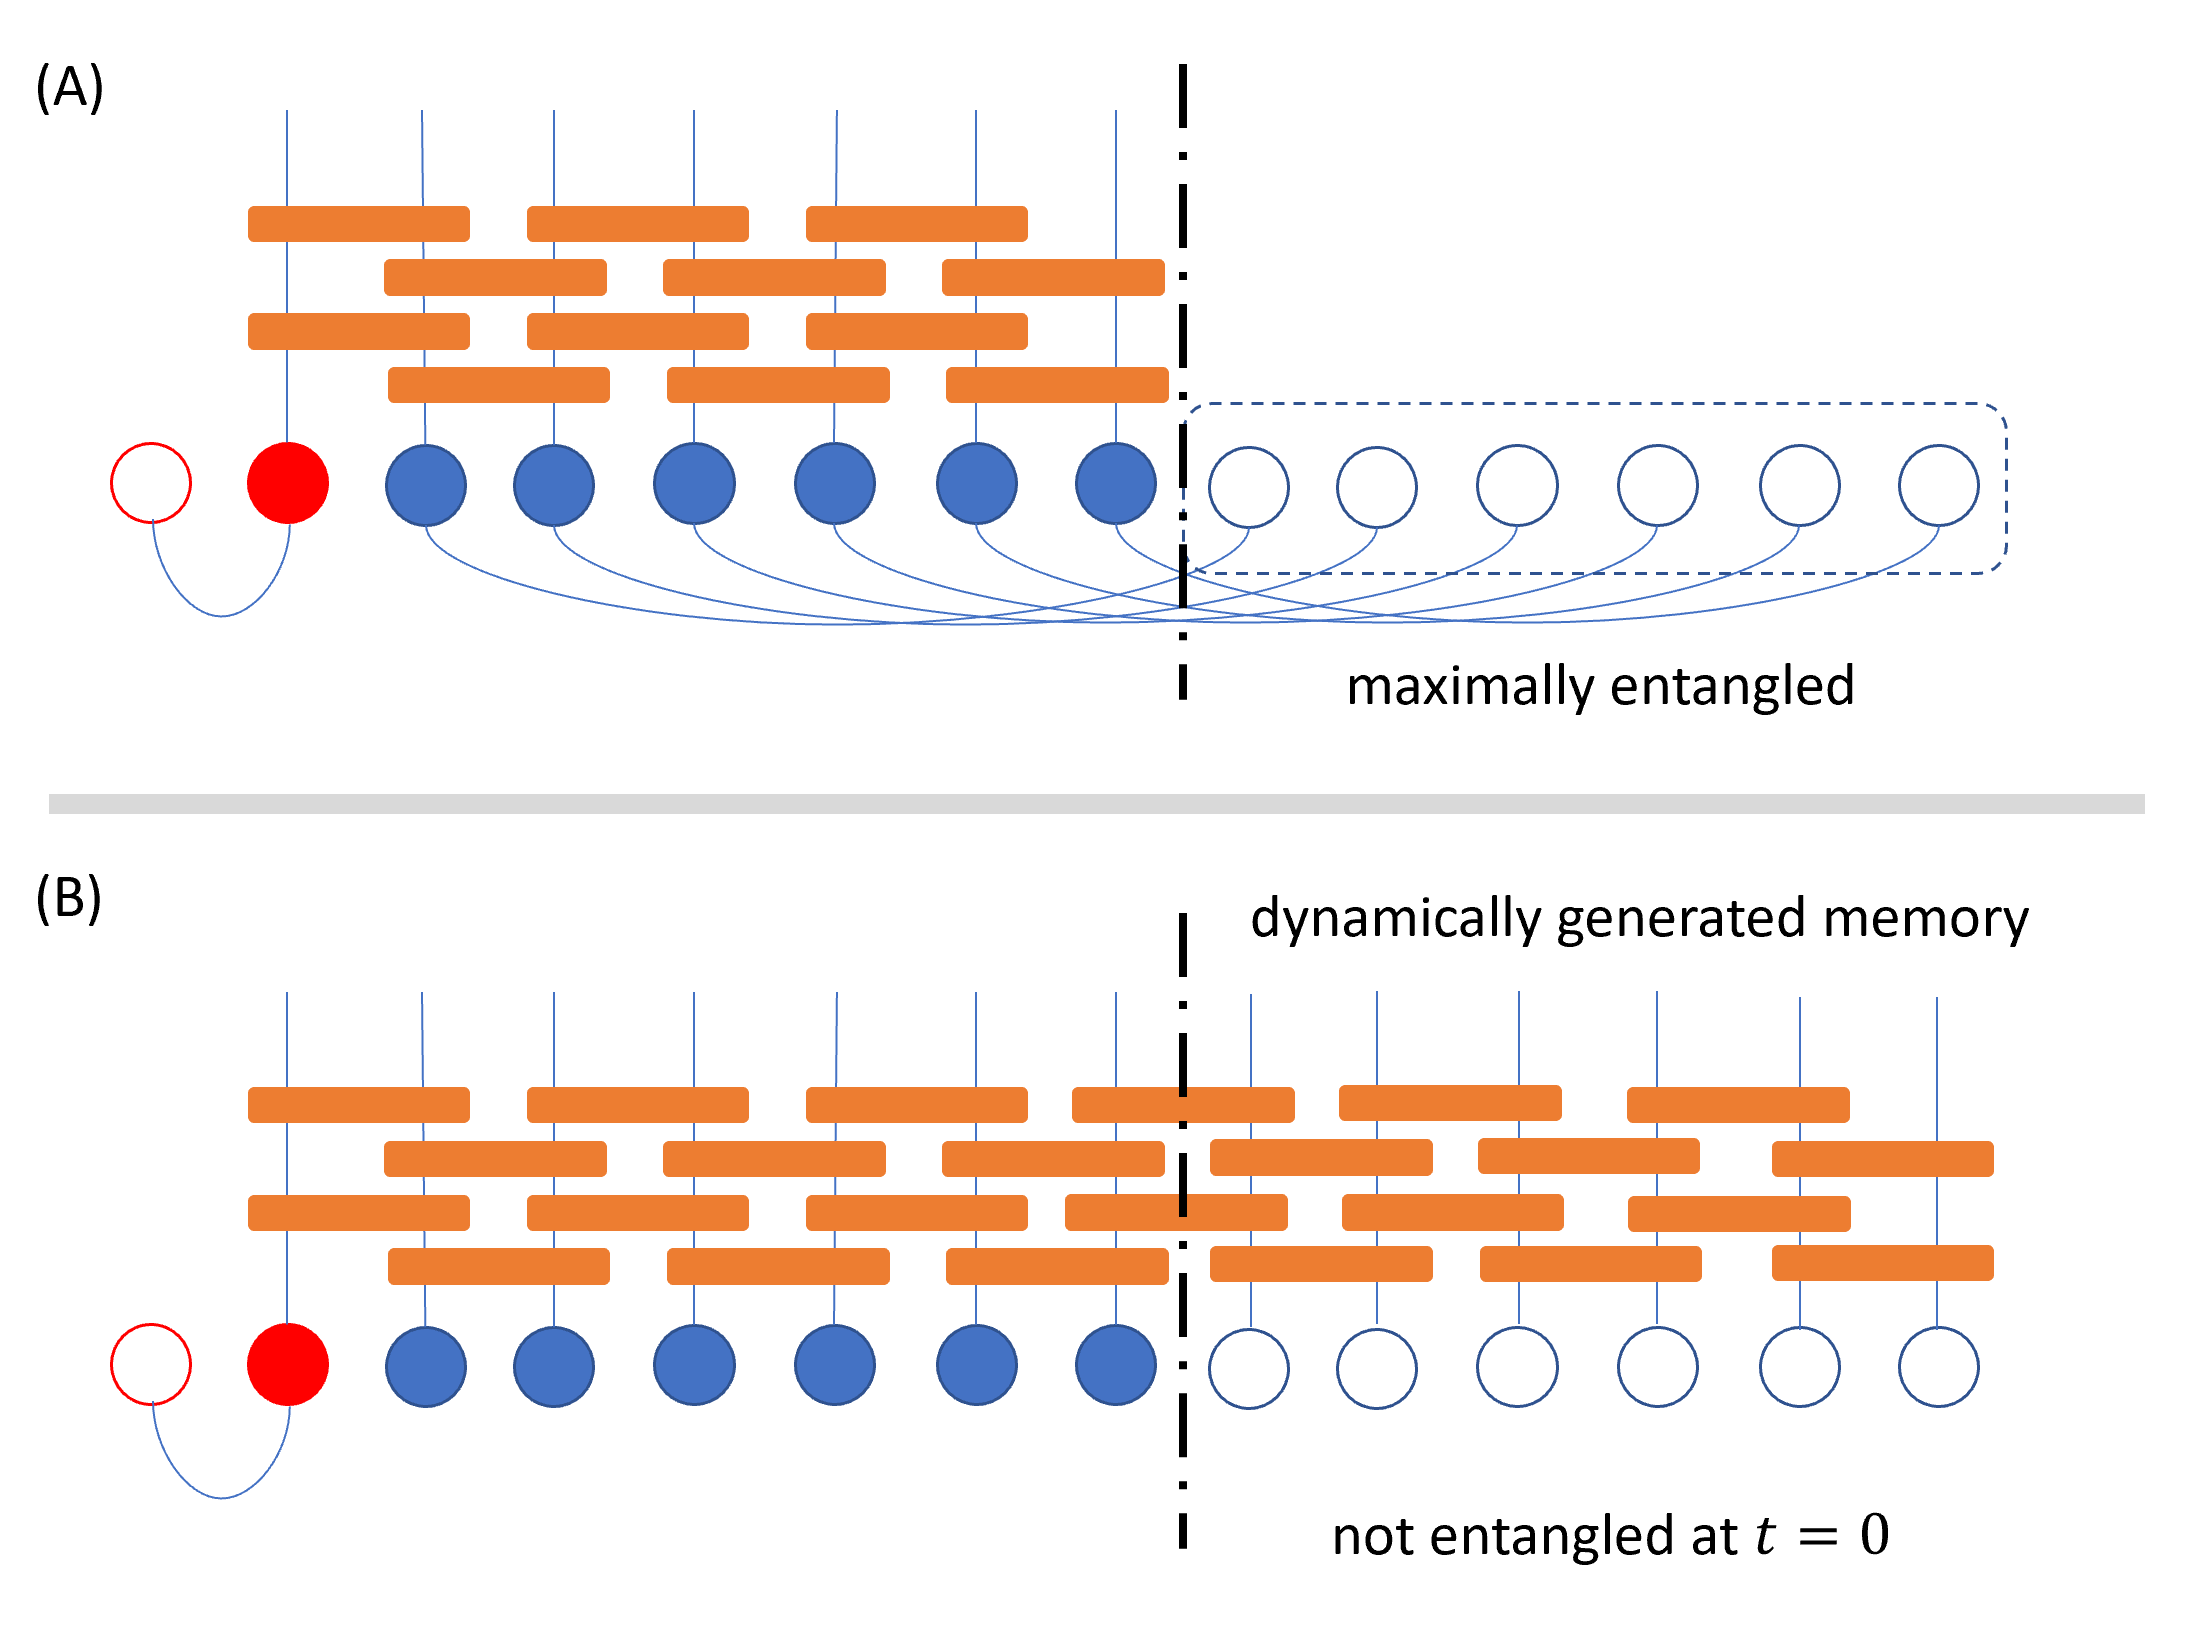
\includegraphics[scale=0.25]{hp_explain}    
    
    \end{center}
    \caption{Our argument vs Hayden Preskill}
    \label{fig:HPExplained}
\end{figure}

\end{minipage}

\end{frame}

% f = 1
\begin{frame}
\frametitle{Quantum Information Argument: $f=1$}

%\begin{minipage}[t]{0.44\linewidth}

\begin{itemize}

\item Consider the case f=0. For simplicity, we will take the total state on the system to be pure.

\item We want to find the (half) width $R(t)$ of the smallest region $A$ from which some initially local entanglement can be recovered.

\item Because we assumed $v_B$ is the fastest length scale, we must have $R(t) \leq v_B t$.

\item On the other hand, if $R(t)<v_B t$, then the information on $A$ is fully scrambled.

\item by HP, because $A$ and $A^{c}$ are maximally entangled, we could recover the entanglement on $A^{c}$ plus a small subsystem of $A$.

\item This cannot be, so $R(t) = v_B t$.

\end{itemize}

%\end{minipage}\hfill
%
%\begin{minipage}[t]{0.55\linewidth}

%\begin{figure}
%    \begin{center}
    
%        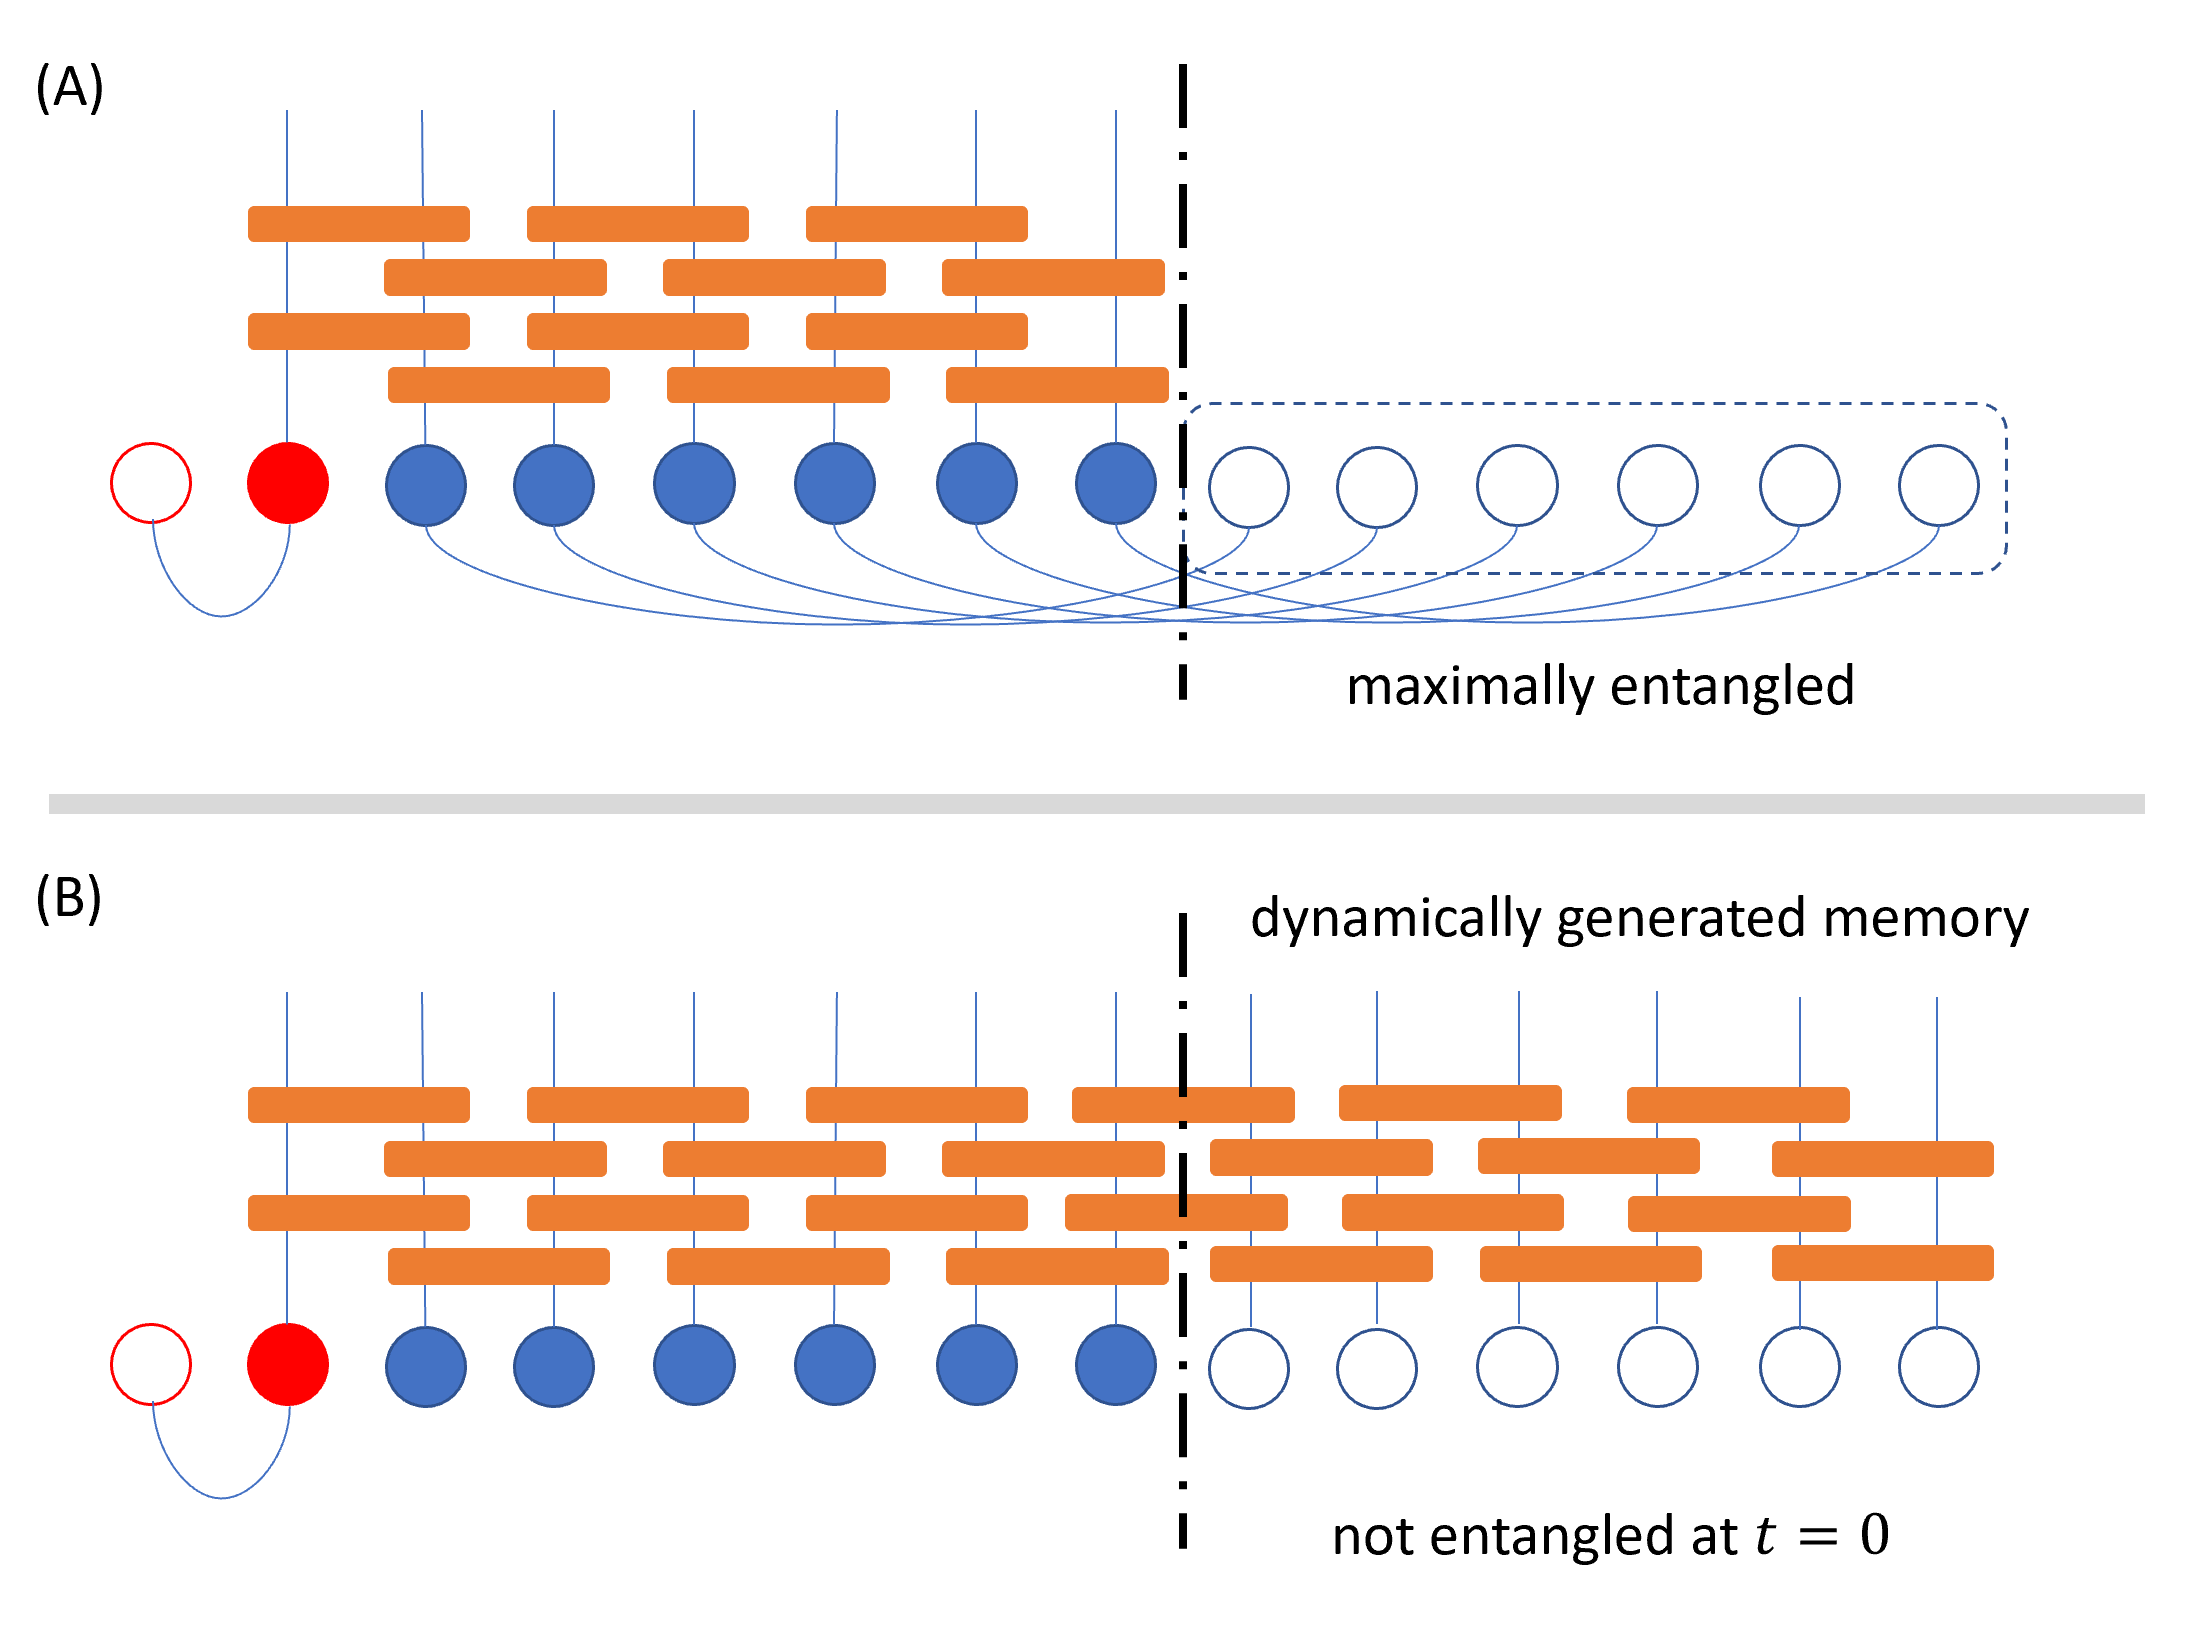
\includegraphics[scale=0.25]{hp_explain}    
    
%    \end{center}
%    \caption{Our argument vs Hayden Preskill}
%    \label{fig:HPExplained2}
%\end{figure}

%\end{minipage}

\end{frame}

% f < 1
\begin{frame}
\frametitle{Quantum Information Argument: $f<1$}

%\begin{minipage}[t]{0.44\linewidth}

\begin{itemize}

\item Now consider $f<1$. If $v_E < (1-f) v_B$, then entanglement is not generated fast enought to run HP as above.

\item The largest system we can run HP on is the one whose entropy has just saturated.

\item The saturation time for a region of size $R$ is given by

\begin{equation}
t_{\text{sat}} = \frac{(1-f) R}{v_E(f)} 
\end{equation}

\item Inverting the above, we find

\begin{equation}
v_I = \frac{v_E(f)}{1-f}
\end{equation}

\end{itemize}

%\end{minipage}\hfill
%
%\begin{minipage}[t]{0.55\linewidth}

%\begin{figure}
%    \begin{center}
    
%        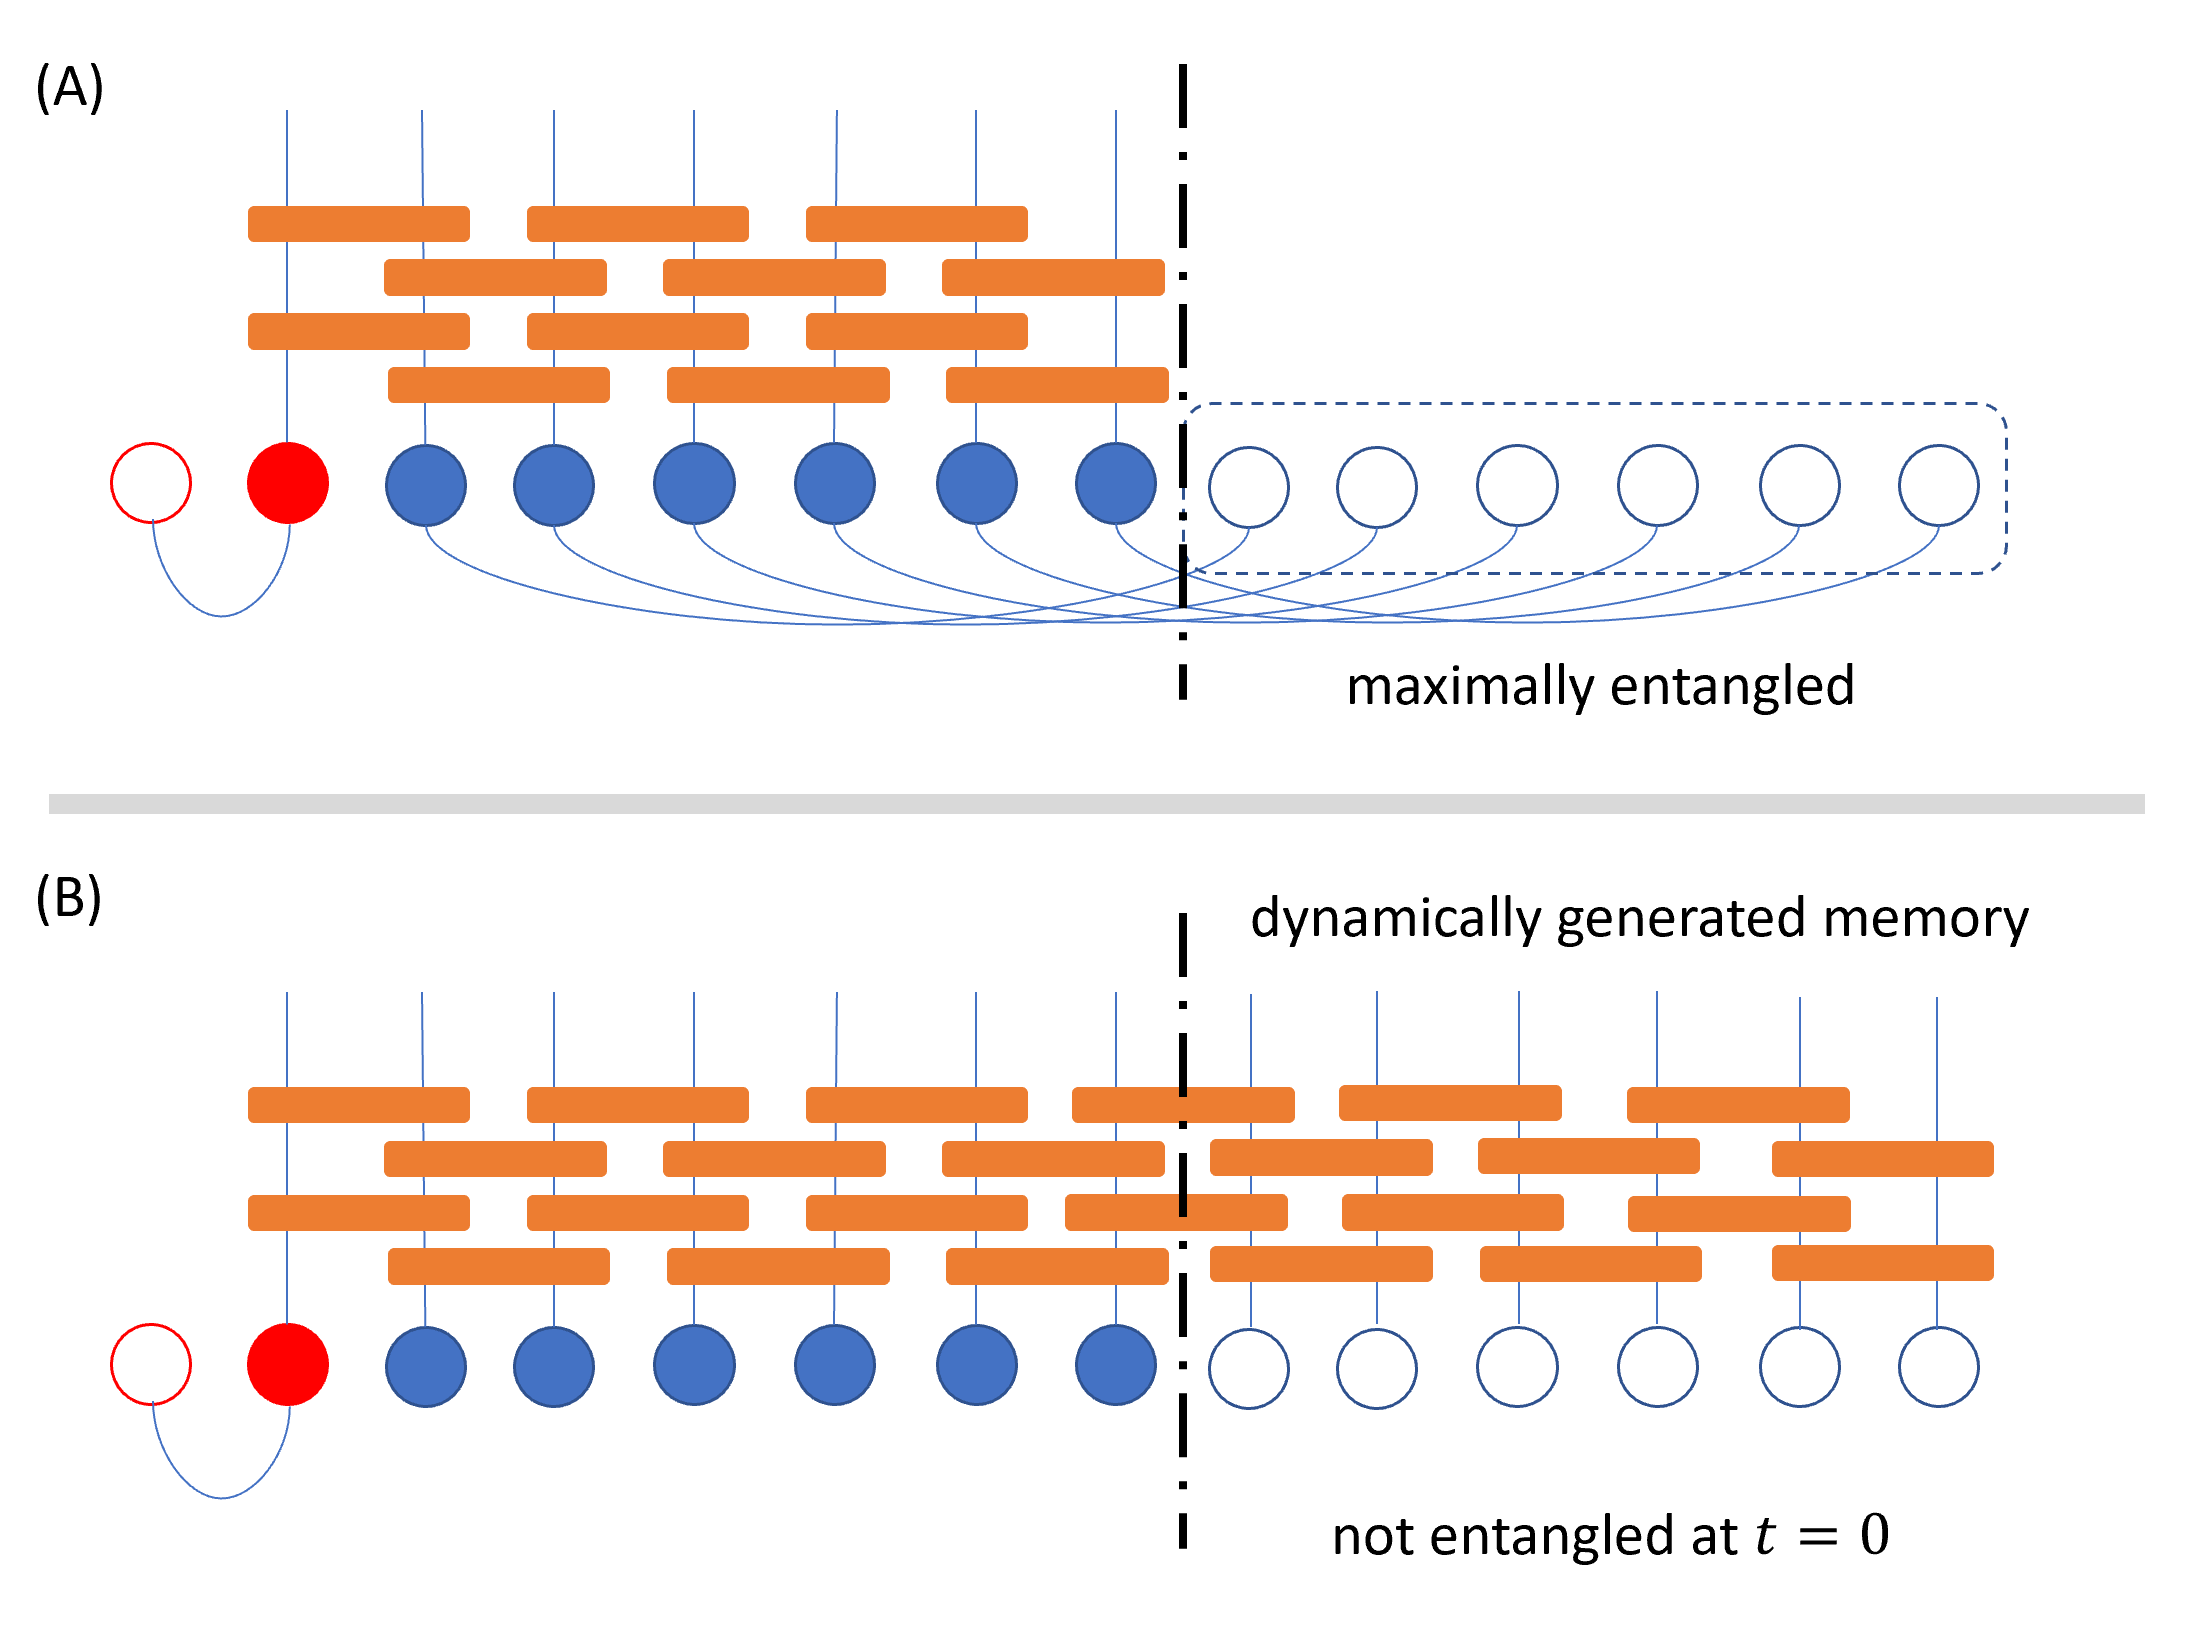
\includegraphics[scale=0.25]{hp_explain}    
    
%    \end{center}
%    \caption{Our argument vs Hayden Preskill}
%    \label{fig:HPExplained2}
%\end{figure}

%\end{minipage}

\end{frame}

% spin chain results
\begin{frame}
\frametitle{Spin Chain Numerics}

\begin{minipage}[t]{0.44\linewidth}

\begin{itemize}

\item Chain of 22 Spins

\item Left most spin initially maximally entangled with reference spin

\item System evolved with a chaotic Hamiltonian

\item At each time step, use mutual information to diagnose the smallest region which can recover this entanglement

\item Small size effects expected, especially for large initial entangling fraction.

\end{itemize}

\end{minipage}\hfill
%
\begin{minipage}[t]{0.55\linewidth}

\begin{figure}
    \begin{center}
    
        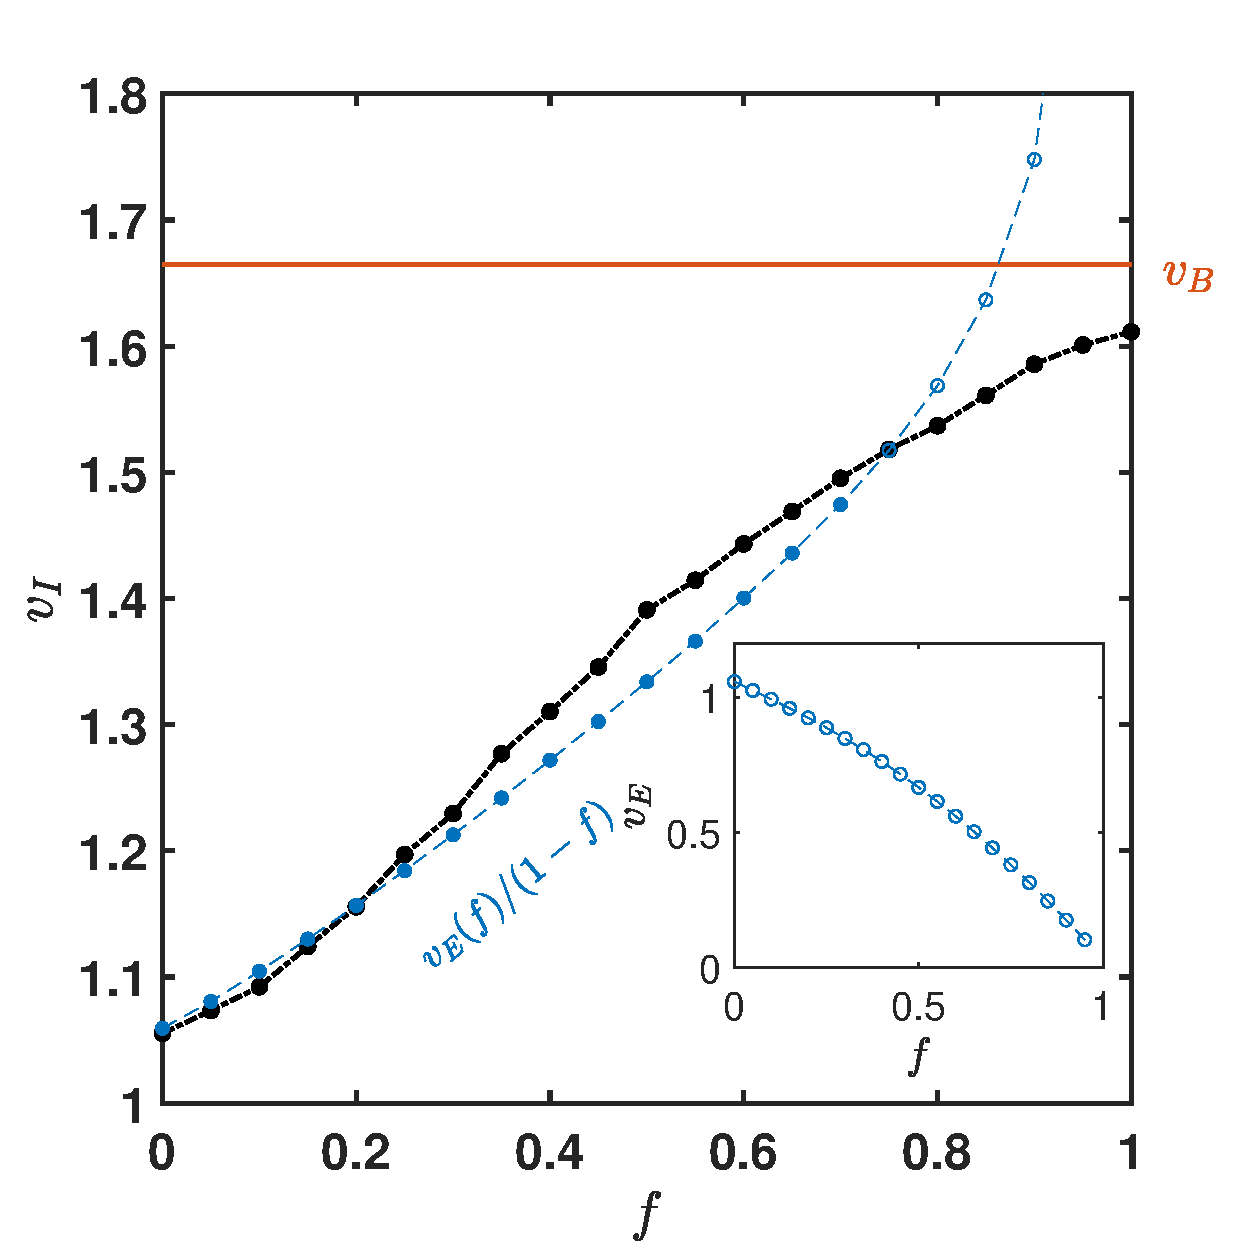
\includegraphics[scale=0.3]{speeds}    
    
    \end{center}
    \caption{$v_I$ vs entanglement fraction for a spin chain:}
    \label{fig:SpinChain}
\end{figure}

\end{minipage}

\end{frame}

% Holography

\begin{frame}
\frametitle{Holographic setup}

\begin{minipage}[t]{0.44\linewidth}

\begin{itemize}

\item We consider either 1 or 2 sided AdS-Vaidya in the thin shell limit.

\item We take the null shock to intersect the boundary at $t = 0$. 

\item We consider a probe particle to fall in the bulk at time  $t_0>0$.

\item The information content of this particle (which we will think of as entanglement with some reference) can be recovered by any entanglement wedge which contains it.

\item We compute the information speed by tracking the smallest region whose entanglement wedge includes the particle at each time.

\item We only consider strip-like regions

\end{itemize}

\end{minipage}\hfill
%
\begin{minipage}[t]{0.55\linewidth}

\begin{figure}
    \begin{center}
    
        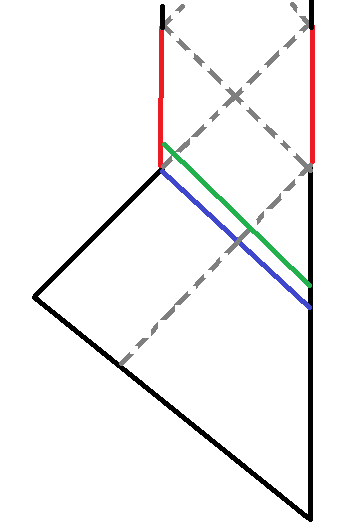
\includegraphics[scale=0.3]{AdSRNVaidyaDiagram}    
    
    \end{center}
    \caption{1-sided AdS-Vaidya}
    \label{fig:Penrose}
\end{figure}

\end{minipage}

\end{frame}


% Entanglement wedges
\begin{frame}
\frametitle{Entanglement wedges}

\begin{minipage}[t]{0.44\linewidth}

\begin{itemize}

\item There are two families of minimal surfaces, those that cross the shock (O type), and those that don't (E type)

\item In the figure on the right:

	\begin{itemize}
	
	\item The blue curve sweeps out the widths of the entangling regions whose 
	E-type surfaces just touch the shock.	
	
	\item The red curve sweeps out regions whose E-type surfaces barely contain the particle
	
	\item The dashed green curve sweeps out the regions at which the E and O type surfaces have equal area, i.e., each $(t, R)$ pair are such that $t = t_{\text{sat}} (R)$.
	
	\end{itemize}
	
\item By the formula for saturation time given above, the green curve gives $v_I = v_E(f)/1-f$ as expected.

\end{itemize}

\end{minipage}\hfill
%
\begin{minipage}[t]{0.55\linewidth}

\begin{figure}
    \begin{center}
    
        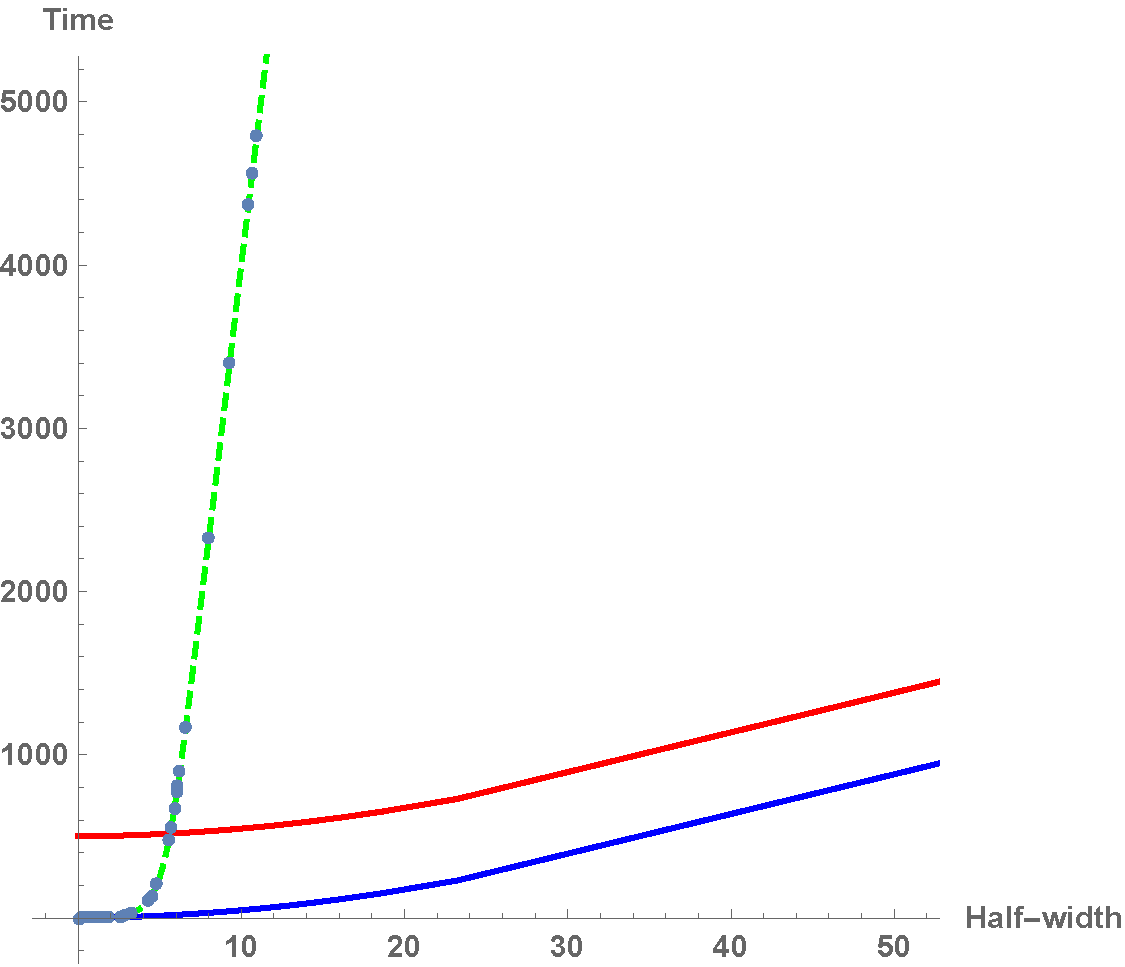
\includegraphics[scale=0.4]{1sidedPhaseDiagram}    
    
    \end{center}
    \caption{Various cones}
    \label{fig:cones}
\end{figure}

\end{minipage}

\end{frame}

\begin{frame}
\frametitle{Numerical Results from Holography}


\begin{minipage}[t]{0.5\linewidth}

\begin{figure}
    \begin{center}
    
        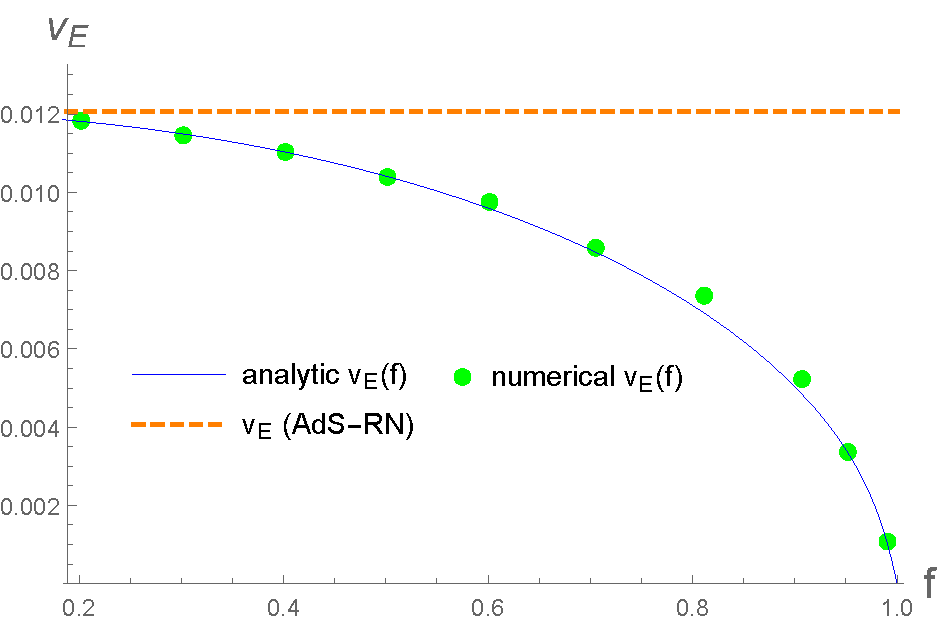
\includegraphics[scale=0.4]{vEvsfholographic}    
    
    \end{center}
    \caption{Numerical results for $v_E$}
    \label{fig:vEFromHolography}
\end{figure}

\end{minipage}\hfill
%
\begin{minipage}[t]{0.5\linewidth}

\begin{figure}
    \begin{center}
    
        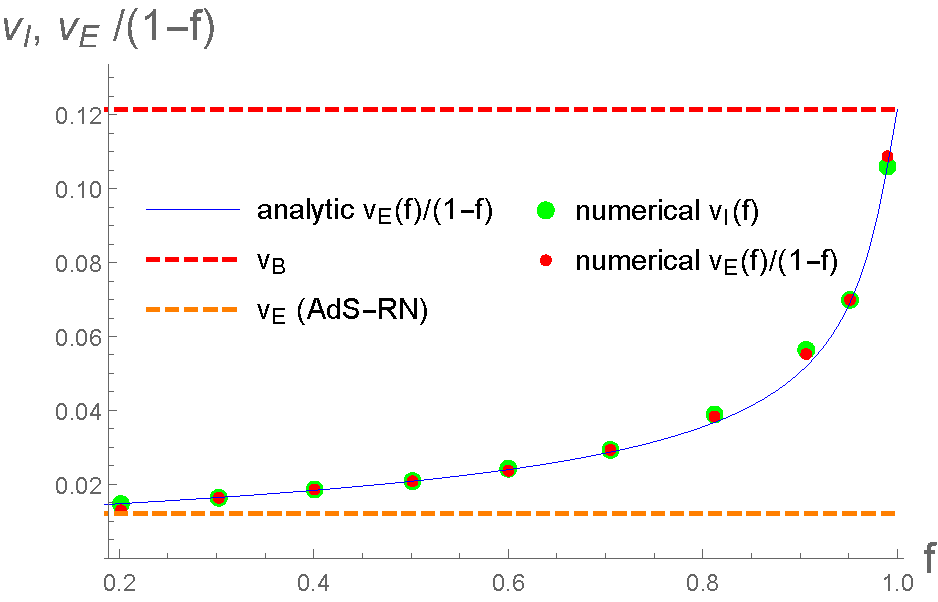
\includegraphics[scale=0.4]{vIvsfholographic}    
    
    \end{center}
    \caption{Numerical results for $v_I$}
    \label{fig:vIFromHolography}
\end{figure}

\end{minipage}

\end{frame}

\begin{frame}
\frametitle{Summary of Results:}

\begin{itemize}

\item Based on our quantum information argument, we seem to have that

\begin{equation}
v_I = \min \left( v_B, \frac{v_E(f)}{1-f} \right)
\end{equation}

\item In all the systems we've checked, we have that $v_E \leq (1-f) v_B$. We have a (not quite rigorous) argument that this is always true, recovering our initial claim.

\item numerical results for a spin chain seem to be in relatively good agreement with this expectation. Due to small size effects, we don't expect exact agreement.

\item The numerical holographic results also seem to be in good agreement with this expectation.
 

\end{itemize}

\end{frame}

\end{document}